\documentclass[a4paper,11pt]{report}

\usepackage{amsmath,amssymb}
\usepackage{fullpage}
\usepackage{graphicx}

\usepackage{bussproofs}
\usepackage{mathpartir}
\usepackage{prooftrees}
\usepackage{color}
\usepackage{rotating}



\usepackage{tikz}
\usetikzlibrary{automata,positioning}
\usetikzlibrary{fit}

\newcommand*\circled[1]{\tikz[baseline=(char.base)]{
    \node[shape=circle,draw,inner sep=2pt] (char) {#1};}}

\makeatletter
\pgfmathdeclarefunction{alpha}{1}{%
  \pgfmathint@{#1}%
  \edef\pgfmathresult{\pgffor@alpha{\pgfmathresult}}%
}

\newcommand*{\until}{U}
\newcommand*{\disj}{\ ,\ }
\newcommand*{\A}{\square}  % Always
\newcommand*{\D}{\diamondsuit} % eventually

\newcommand*{\Pq}{(\top,\bot)}
\newcommand*{\pQ}{(\bot,\top)}
\newcommand*{\PQ}{(\top,\top)}
\newcommand*{\pq}{(\bot,\bot)}


% tikz
\usepackage{tikz}
\usetikzlibrary{snakes}



\author{Sylvain Julmy}
\date{\today}

\setlength{\parindent}{0pt}
\setlength{\parskip}{2.5pt}

\begin{document}

\begin{center}
  \Large{
    Automata on Infinite Structure\\
    Fall 2018
  }
  
  \noindent\makebox[\linewidth]{\rule{\linewidth}{0.4pt}}
  Exercice Sheet 6

  \vspace*{1.4cm}

  Author : Sylvain Julmy
  \noindent\makebox[\linewidth]{\rule{\linewidth}{0.4pt}}

  \begin{flushleft}
    Professor : Ultes-Nitsche Ulrich
    
    Assistant : Stammet Christophe
  \end{flushleft}

  \noindent\makebox[\linewidth]{\rule{\textwidth}{1pt}}
\end{center}

\section*{Exercise 1}

\begin{center}
  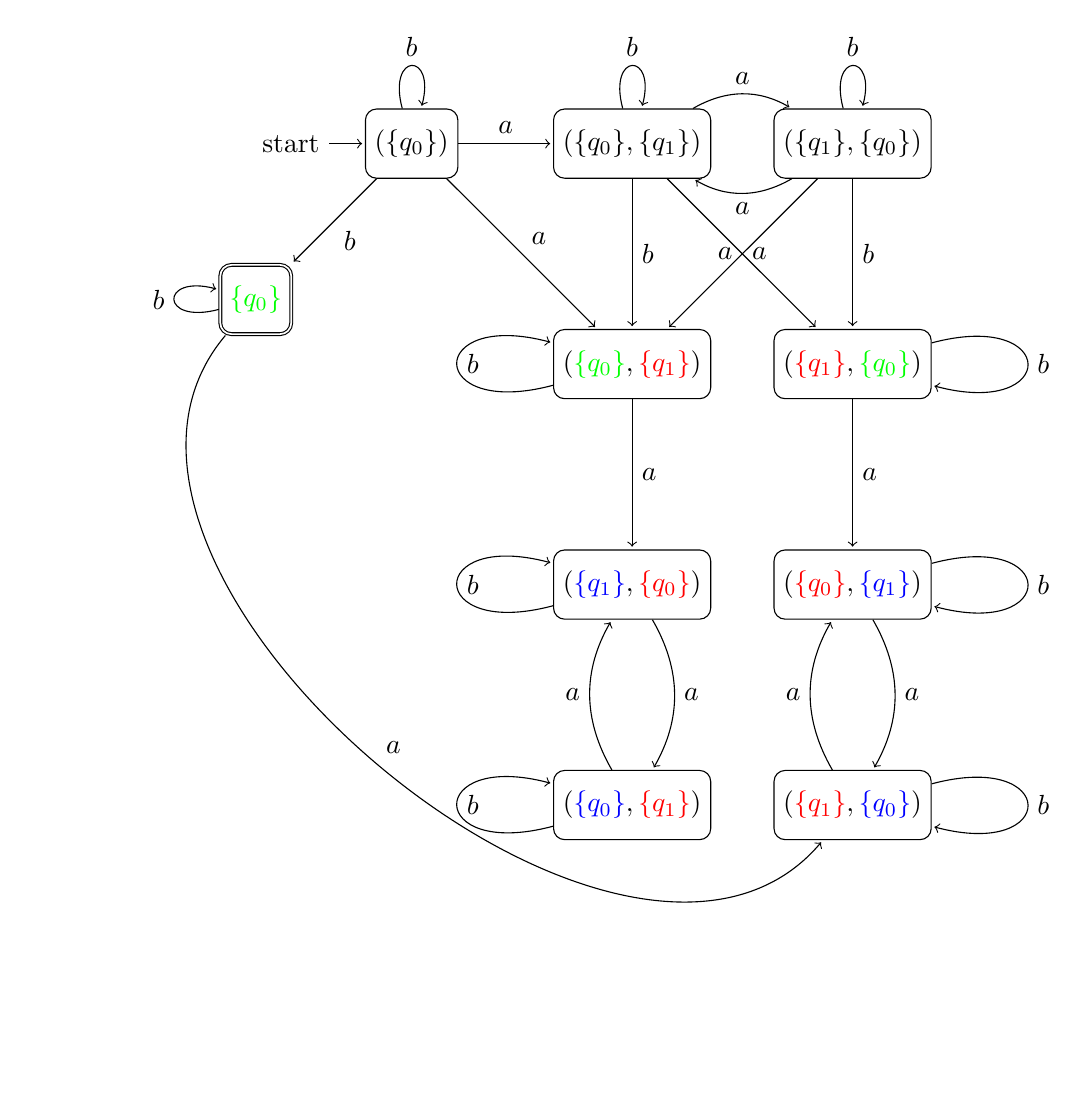
\begin{tikzpicture}[shorten >=1pt,node distance=2.8cm,on grid,auto]
    \tikzset{rounded/.style={draw,rectangle,rounded corners}}
    \node[state,rounded,initial] (q0) {$(\{q_0\})$};
    \node[state,rounded] (q0q1) [right = of q0] {$(\{q_0\},\{q_1\})$};
    \node[state,rounded] (q1q0) [right = of q0q1] {$(\{q_1\},\{q_0\})$};
    
    \node[state,rounded] (q0q1b) [below = of q0q1] {$(\textcolor{green}{\{q_0\}},\textcolor{red}{\{q_1\}})$};
    \node[state,rounded] (q1q0b) [below = of q1q0] {$(\textcolor{red}{\{q_1\}},\textcolor{green}{\{q_0\}})$};
    
    \node[state,rounded] (q1q0c) [below = of q0q1b] {$(\textcolor{blue}{\{q_1\}},\textcolor{red}{\{q_0\}})$};
    \node[state,rounded] (q0q1c) [below = of q1q0c] {$(\textcolor{blue}{\{q_0\}},\textcolor{red}{\{q_1\}})$};
    
    \node[state,rounded] (q0q1d) [below = of q1q0b] {$(\textcolor{red}{\{q_0\}},\textcolor{blue}{\{q_1\}})$};
    \node[state,rounded] (q1q0d) [below = of q0q1d] {$(\textcolor{red}{\{q_1\}},\textcolor{blue}{\{q_0\}})$};

    \node[state,rounded,accepting] (q0b) [below left = of q0] {$\textcolor{green}{\{q_0\}}$};
    
    \path[->]
    (q0)
    edge [] node [] {$a$} (q0q1)
    edge [loop above] node [] {$b$} ()
    edge [] node [] {$a$} (q0q1b)
    edge [] node [] {$b$} (q0b)
    (q0q1)
    edge [bend left] node [] {$a$} (q1q0)
    edge [loop above] node [] {$b$} ()
    edge [] node [right] {$a$} (q1q0b)
    edge [] node [] {$b$} (q0q1b)
    (q1q0)
    edge [bend left] node [] {$a$} (q0q1)
    edge [loop above] node [] {$b$} ()
    edge [] node [] {$b$} (q1q0b)
    edge [] node [left] {$a$} (q0q1b)
    (q0q1b)
    edge [] node {$a$} (q1q0c)
    edge [loop left] node [right] {$b$} ()
    (q1q0c)
    edge [bend left] node {$a$} (q0q1c)
    edge [loop left] node [right] {$b$} ()
    (q0q1c)
    edge [bend left] node {$a$} (q1q0c)
    edge [loop left] node [right] {$b$} ()
    (q1q0b)
    edge [] node {$a$} (q0q1d)
    edge [loop right] node {$b$} ()
    (q0q1d)
    edge [bend left] node {$a$} (q1q0d)
    edge [loop right] node {$b$} ()
    (q1q0d)
    edge [bend left] node {$a$} (q0q1d)
    edge [loop right] node {$b$} ()
    (q0b)
    edge [loop left] node {$b$} ()
    edge [bend right = 90] node {$a$} (q1q0d)
    ;
  \end{tikzpicture}
\end{center}

\newpage

\section*{Exercise 2}

{\centering
  \begin{turn}{90}
    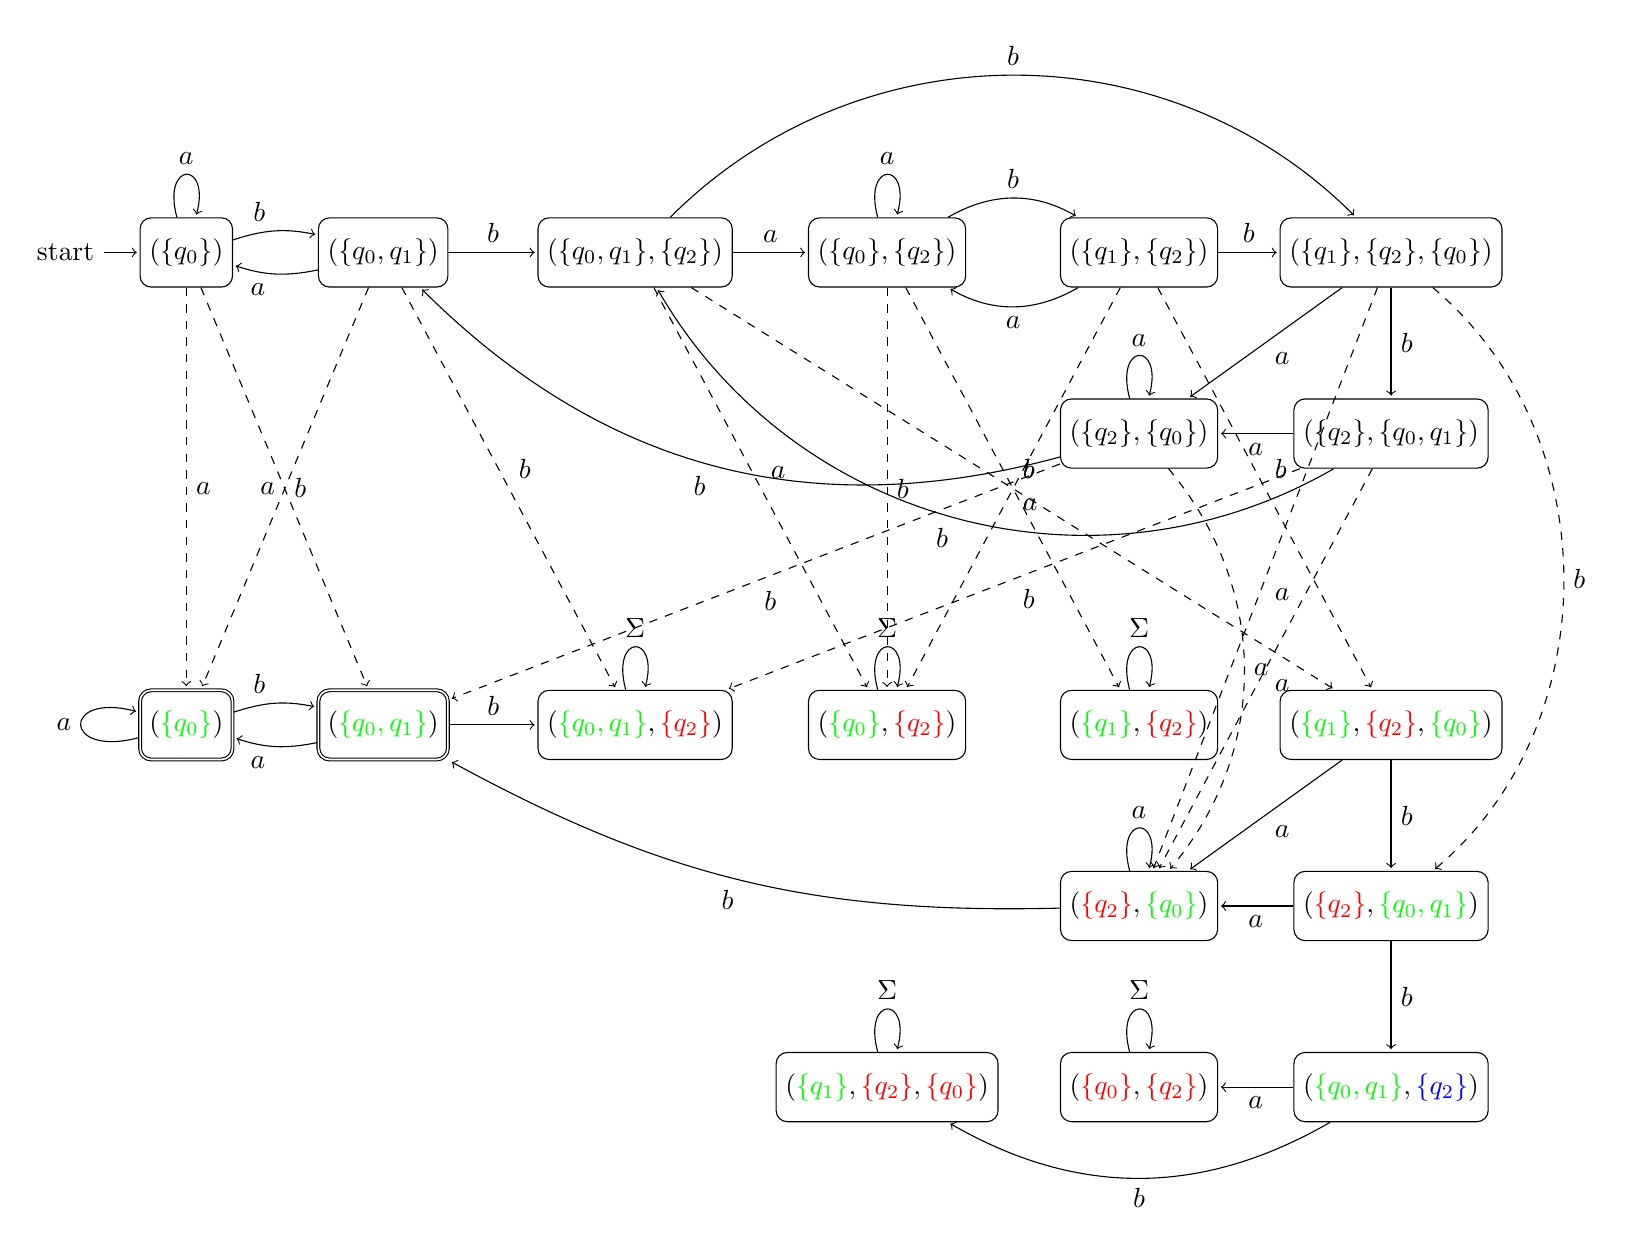
\begin{tikzpicture}[shorten >=1pt,node distance=2cm,on grid,auto]
      \tikzset{rounded/.style={draw,rectangle,rounded corners}}
      
      \node[state,rounded,initial] (q0) {$(\{q_0\})$};
      \node[state,rounded] (q0q1) [right = 2.5cm of q0] {$(\{q_0,q_1\})$};
      \node[state,rounded] (q0q1q2) [right = 3.2cm of q0q1] {$(\{q_0,q_1\},\{q_2\})$};
      \node[state,rounded] (q0q2) [right = 3.2cm of q0q1q2] {$(\{q_0\},\{q_2\})$};
      \node[state,rounded] (q1q2) [right = 3.2cm of q0q2] {$(\{q_1\},\{q_2\})$};
      \node[state,rounded] (q1q2q0) [right = 3.2cm of q1q2] {$(\{q_1\},\{q_2\},\{q_0\})$};
      \node[state,rounded] (q2q0) [below = 2.3cm of q1q2] {$(\{q_2\},\{q_0\})$};
      \node[state,rounded] (q2q0q1) [below = 2.3cm of q1q2q0] {$(\{q_2\},\{q_0,q_1\})$};
      
      \node[state,rounded,accepting] (q0b) [below = 6cm of q0] {$(\textcolor{green}{\{q_0\}})$};
      \node[state,rounded,accepting] (q0q1b) [right = 2.5cm of q0b] {$(\textcolor{green}{\{q_0,q_1\}})$};
      \node[state,rounded] (q0q1q2b) [right = 3.2cm of q0q1b] {$(\textcolor{green}{\{q_0,q_1\}},\textcolor{red}{\{q_2\}})$};
      \node[state,rounded] (q0q2b) [right = 3.2cm of q0q1q2b] {$(\textcolor{green}{\{q_0\}},\textcolor{red}{\{q_2\}})$};
      \node[state,rounded] (q1q2b) [right = 3.2cm of q0q2b] {$(\textcolor{green}{\{q_1\}},\textcolor{red}{\{q_2\}})$};
      \node[state,rounded] (q1q2q0b) [right = 3.2cm of q1q2b] {$(\textcolor{green}{\{q_1\}},\textcolor{red}{\{q_2\}},\textcolor{green}{\{q_0\}})$};
      \node[state,rounded] (q2q0b) [below = 2.3cm of q1q2b] {$(\textcolor{red}{\{q_2\}},\textcolor{green}{\{q_0\}})$};
      \node[state,rounded] (q2q0q1b) [below = 2.3cm of q1q2q0b] {$(\textcolor{red}{\{q_2\}},\textcolor{green}{\{q_0,q_1\}})$};
      
      \node[state,rounded] (q0q1q2c) [below = 2.3cm of q2q0q1b] {$(\textcolor{green}{\{q_0,q_1\}},\textcolor{blue}{\{q_2\}})$};
      \node[state,rounded] (q0q2c) [left = 3.2cm of q0q1q2c] {$(\textcolor{red}{\{q_0\}},\textcolor{red}{\{q_2\}})$};
      \node[state,rounded] (q1q2q0c) [left = 3.2cm of q0q2c] {$(\textcolor{green}{\{q_1\}},\textcolor{red}{\{q_2\}},\textcolor{red}{\{q_0\}})$};
      
      \path[->]
      (q0)
      edge [loop above] node [] {$a$} ()
      edge [dashed] node [] {$a$} (q0b)
      edge [bend left = 15] node [] {$b$} (q0q1)
      edge [dashed] node [right] {$b$} (q0q1b)
      (q0q1)
      edge [bend left = 15] node [] {$a$} (q0)
      edge [] node [] {$b$} (q0q1q2)
      edge [dashed] node [left] {$a$} (q0b)
      edge [dashed] node [] {$b$} (q0q1q2b)
      (q0q1q2)
      edge [] node [] {$a$} (q0q2)
      edge [dashed] node [] {$a$} (q0q2b)
      edge [bend left = 45] node [] {$b$} (q1q2q0)
      edge [dashed] node [] {$b$} (q1q2q0b)
      (q0q2)
      edge [loop above] node [] {$a$} ()
      edge [dashed] node [] {$b$} (q0q2b)
      edge [bend left] node [] {$b$} (q1q2)
      edge [dashed] node [] {$b$} (q1q2b)
      (q1q2)
      edge [bend left] node [] {$a$} (q0q2)
      edge [dashed] node [] {$a$} (q0q2b)
      edge [] node [] {$b$} (q1q2q0)
      edge [dashed] node [] {$b$} (q1q2q0b)
      (q1q2q0)
      edge [] node [] {$a$} (q2q0)
      edge [] node [] {$b$} (q2q0q1)
      edge [dashed] node [] {$a$} (q2q0b)
      edge [dashed,bend left = 50] node [] {$b$} (q2q0q1b)
      (q2q0)
      edge [loop above] node [] {$a$} ()
      edge [dashed,bend left = 40] node [] {$a$} (q2q0b)
      edge [bend left] node [] {$b$} (q0q1)
      edge [dashed] node [] {$b$} (q0q1b)
      (q2q0q1)
      edge [] node [] {$a$} (q2q0)
      edge [dashed] node [] {$a$} (q2q0b)
      edge [bend left = 45] node [] {$b$} (q0q1q2)
      edge [dashed] node [] {$b$} (q0q1q2b)
      (q0b)
      edge [loop left] node [] {$a$} ()
      edge [bend left = 15] node [] {$b$} (q0q1b)
      (q0q1b)
      edge [bend left = 15] node [] {$a$} (q0b)
      edge [] node [] {$b$} (q0q1q2b)
      (q0q1q2b)
      edge [loop above] node [] {$\Sigma$} ()
      (q0q2b)
      edge [loop above] node [] {$\Sigma$} ()
      (q1q2b)
      edge [loop above] node [] {$\Sigma$} ()
      (q1q2q0b)
      edge [] node [] {$a$} (q2q0b)
      edge [] node [] {$b$} (q2q0q1b)
      (q2q0b)
      edge [loop above] node [] {$a$} ()
      edge [bend left = 15] node [] {$b$} (q0q1b)
      (q2q0q1b)
      edge [] node [] {$a$} (q2q0b)
      edge [] node [] {$b$} (q0q1q2c)
      (q0q1q2c)
      edge [] node [] {$a$} (q0q2c)
      edge [bend left] node [] {$b$} (q1q2q0c)
      (q0q2c)
      edge [loop above] node [] {$\Sigma$} ()
      (q1q2q0c)
      edge [loop above] node [] {$\Sigma$} ()
      ;
    \end{tikzpicture}
  } % centering
\end{turn}


\newpage

The same automaton, but without the dashed transition :

{\centering
  \begin{turn}{90}
    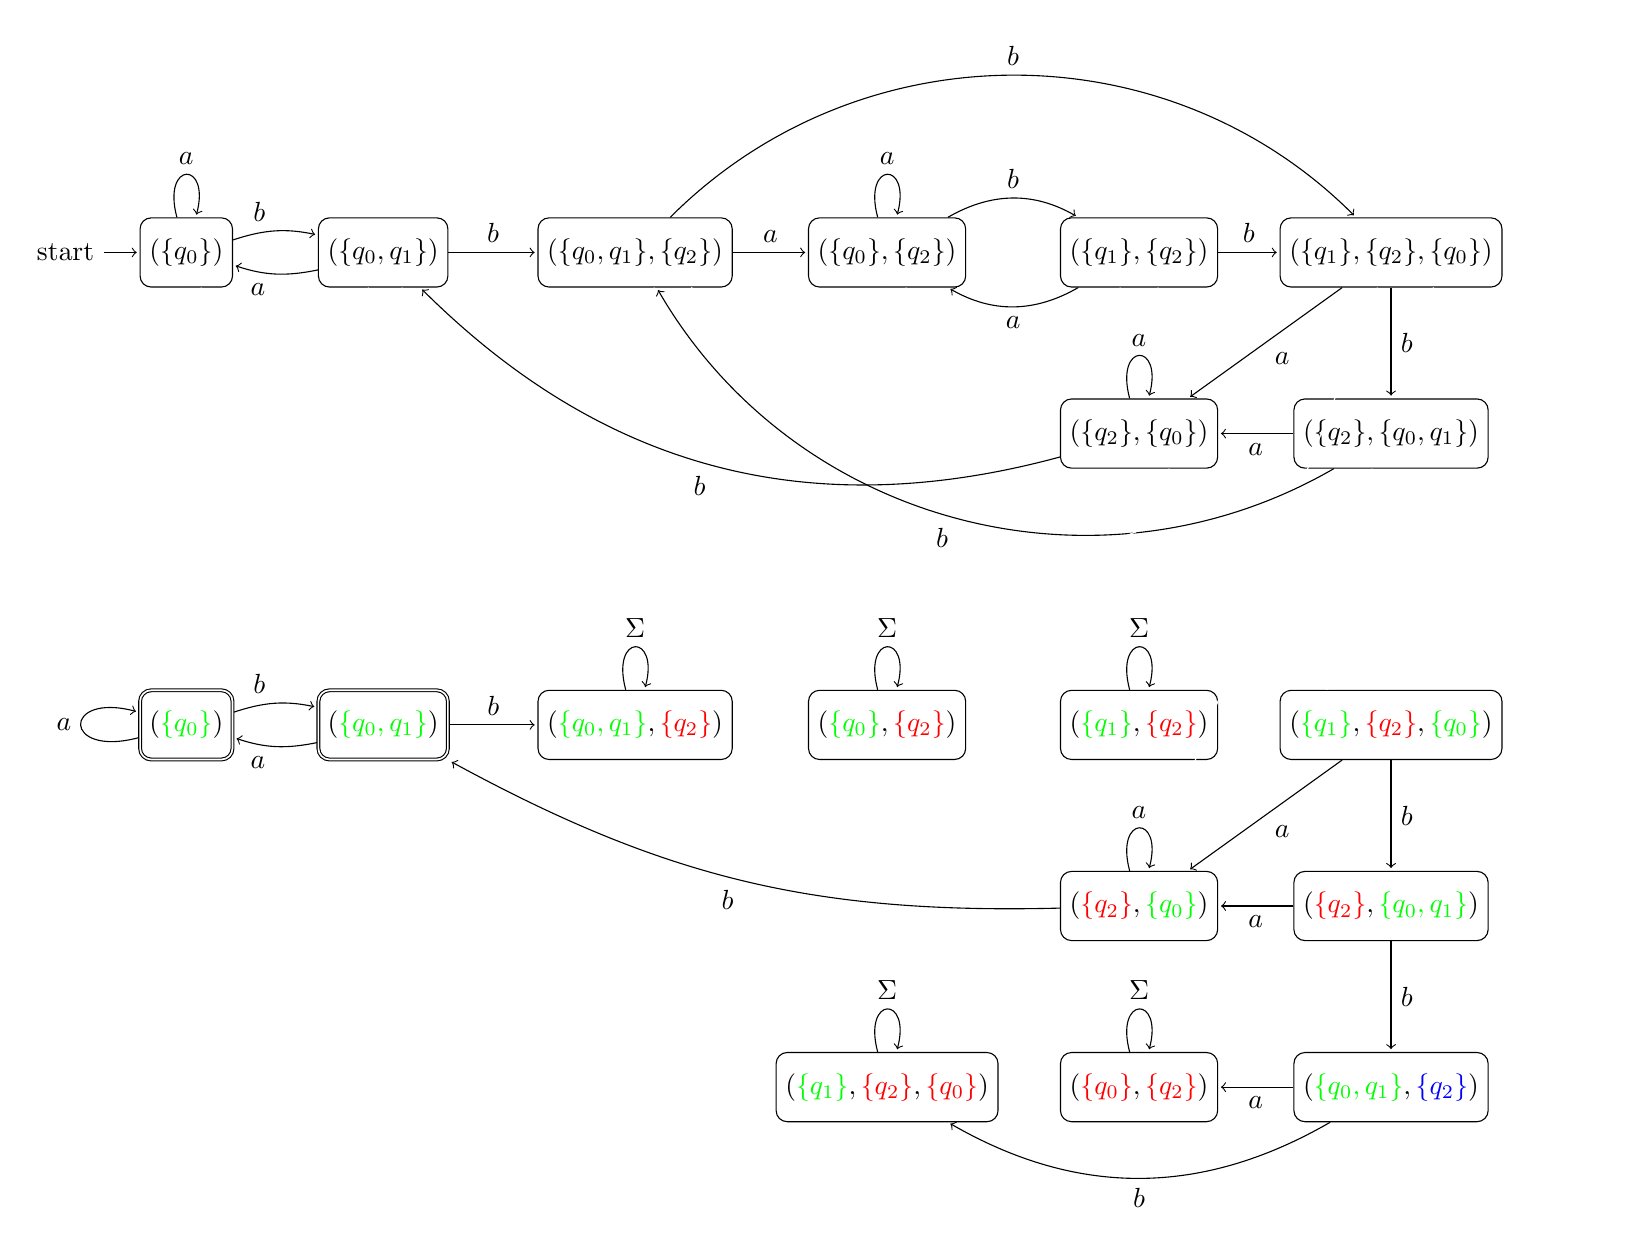
\begin{tikzpicture}[shorten >=1pt,node distance=2cm,on grid,auto]
      \tikzset{rounded/.style={draw,rectangle,rounded corners}}
      
      \node[state,rounded,initial] (q0) {$(\{q_0\})$};
      \node[state,rounded] (q0q1) [right = 2.5cm of q0] {$(\{q_0,q_1\})$};
      \node[state,rounded] (q0q1q2) [right = 3.2cm of q0q1] {$(\{q_0,q_1\},\{q_2\})$};
      \node[state,rounded] (q0q2) [right = 3.2cm of q0q1q2] {$(\{q_0\},\{q_2\})$};
      \node[state,rounded] (q1q2) [right = 3.2cm of q0q2] {$(\{q_1\},\{q_2\})$};
      \node[state,rounded] (q1q2q0) [right = 3.2cm of q1q2] {$(\{q_1\},\{q_2\},\{q_0\})$};
      \node[state,rounded] (q2q0) [below = 2.3cm of q1q2] {$(\{q_2\},\{q_0\})$};
      \node[state,rounded] (q2q0q1) [below = 2.3cm of q1q2q0] {$(\{q_2\},\{q_0,q_1\})$};
      
      \node[state,rounded,accepting] (q0b) [below = 6cm of q0] {$(\textcolor{green}{\{q_0\}})$};
      \node[state,rounded,accepting] (q0q1b) [right = 2.5cm of q0b] {$(\textcolor{green}{\{q_0,q_1\}})$};
      \node[state,rounded] (q0q1q2b) [right = 3.2cm of q0q1b] {$(\textcolor{green}{\{q_0,q_1\}},\textcolor{red}{\{q_2\}})$};
      \node[state,rounded] (q0q2b) [right = 3.2cm of q0q1q2b] {$(\textcolor{green}{\{q_0\}},\textcolor{red}{\{q_2\}})$};
      \node[state,rounded] (q1q2b) [right = 3.2cm of q0q2b] {$(\textcolor{green}{\{q_1\}},\textcolor{red}{\{q_2\}})$};
      \node[state,rounded] (q1q2q0b) [right = 3.2cm of q1q2b] {$(\textcolor{green}{\{q_1\}},\textcolor{red}{\{q_2\}},\textcolor{green}{\{q_0\}})$};
      \node[state,rounded] (q2q0b) [below = 2.3cm of q1q2b] {$(\textcolor{red}{\{q_2\}},\textcolor{green}{\{q_0\}})$};
      \node[state,rounded] (q2q0q1b) [below = 2.3cm of q1q2q0b] {$(\textcolor{red}{\{q_2\}},\textcolor{green}{\{q_0,q_1\}})$};
      
      \node[state,rounded] (q0q1q2c) [below = 2.3cm of q2q0q1b] {$(\textcolor{green}{\{q_0,q_1\}},\textcolor{blue}{\{q_2\}})$};
      \node[state,rounded] (q0q2c) [left = 3.2cm of q0q1q2c] {$(\textcolor{red}{\{q_0\}},\textcolor{red}{\{q_2\}})$};
      \node[state,rounded] (q1q2q0c) [left = 3.2cm of q0q2c] {$(\textcolor{green}{\{q_1\}},\textcolor{red}{\{q_2\}},\textcolor{red}{\{q_0\}})$};
      
      \path[->]
      (q0)
      edge [loop above] node [] {$a$} ()
      edge [white] node [] {$a$} (q0b)
      edge [bend left = 15] node [] {$b$} (q0q1)
      edge [white] node [right] {$b$} (q0q1b)
      (q0q1)
      edge [bend left = 15] node [] {$a$} (q0)
      edge [] node [] {$b$} (q0q1q2)
      edge [white] node [left] {$a$} (q0b)
      edge [white] node [] {$b$} (q0q1q2b)
      (q0q1q2)
      edge [] node [] {$a$} (q0q2)
      edge [white] node [] {$a$} (q0q2b)
      edge [bend left = 45] node [] {$b$} (q1q2q0)
      edge [white] node [] {$b$} (q1q2q0b)
      (q0q2)
      edge [loop above] node [] {$a$} ()
      edge [white] node [] {$b$} (q0q2b)
      edge [bend left] node [] {$b$} (q1q2)
      edge [white] node [] {$b$} (q1q2b)
      (q1q2)
      edge [bend left] node [] {$a$} (q0q2)
      edge [white] node [] {$a$} (q0q2b)
      edge [] node [] {$b$} (q1q2q0)
      edge [white] node [] {$b$} (q1q2q0b)
      (q1q2q0)
      edge [] node [] {$a$} (q2q0)
      edge [] node [] {$b$} (q2q0q1)
      edge [white] node [] {$a$} (q2q0b)
      edge [white,bend left = 50] node [] {$b$} (q2q0q1b)
      (q2q0)
      edge [loop above] node [] {$a$} ()
      edge [white,bend left = 40] node [] {$a$} (q2q0b)
      edge [bend left] node [] {$b$} (q0q1)
      edge [white] node [] {$b$} (q0q1b)
      (q2q0q1)
      edge [] node [] {$a$} (q2q0)
      edge [white] node [] {$a$} (q2q0b)
      edge [bend left = 45] node [] {$b$} (q0q1q2)
      edge [white] node [] {$b$} (q0q1q2b)
      (q0b)
      edge [loop left] node [] {$a$} ()
      edge [bend left = 15] node [] {$b$} (q0q1b)
      (q0q1b)
      edge [bend left = 15] node [] {$a$} (q0b)
      edge [] node [] {$b$} (q0q1q2b)
      (q0q1q2b)
      edge [loop above] node [] {$\Sigma$} ()
      (q0q2b)
      edge [loop above] node [] {$\Sigma$} ()
      (q1q2b)
      edge [loop above] node [] {$\Sigma$} ()
      (q1q2q0b)
      edge [] node [] {$a$} (q2q0b)
      edge [] node [] {$b$} (q2q0q1b)
      (q2q0b)
      edge [loop above] node [] {$a$} ()
      edge [bend left = 15] node [] {$b$} (q0q1b)
      (q2q0q1b)
      edge [] node [] {$a$} (q2q0b)
      edge [] node [] {$b$} (q0q1q2c)
      (q0q1q2c)
      edge [] node [] {$a$} (q0q2c)
      edge [bend left] node [] {$b$} (q1q2q0c)
      (q0q2c)
      edge [loop above] node [] {$\Sigma$} ()
      (q1q2q0c)
      edge [loop above] node [] {$\Sigma$} ()
      ;
    \end{tikzpicture}
  } % centering
\end{turn}




\end{document}